These sensors will enhance the safe and effective use of the RV8 robot for users. Firstly, the vision sensor assists the robot in aiming at targets. Secondly, the E-stop feature halts the system whenever a user presses the button or it's triggered by the computer. Lastly, the Gate sensor indicates whether the case gate is open or closed. Hence, all the inputs will be transferred to the PLC to initiate actions.


\subsection{Layer Hardware}
The sensors, including the vision sensor, e-stops, and gate, are connected to the programmable logical controller (PLC) via wires. They continuously transmit input values to the PLC, enabling the system to make informed decisions about subsequent actions.

\subsection{Layer Operating System}
RT ToolBox 3 Pro can be installed on both Windows 11 and Windows 10 operating systems.

\subsection{Layer Software Dependencies}
RT ToolBox 3, which controls the robot, will be used to facilitate the movement of the robot arm.

\subsection{Vision Sensor}
Vision sensors serve multiple purposes, including aiming at a target and tracing its movement. Additionally, it incorporates a safety feature: if there is any movement detected by the camera, it will automatically halt the program to ensure safety. This sensor will be mounted on the robot arm, enabling it to adjust its position by manipulating the robot arm's movements.

\begin{figure}[h!]
	\centering
 	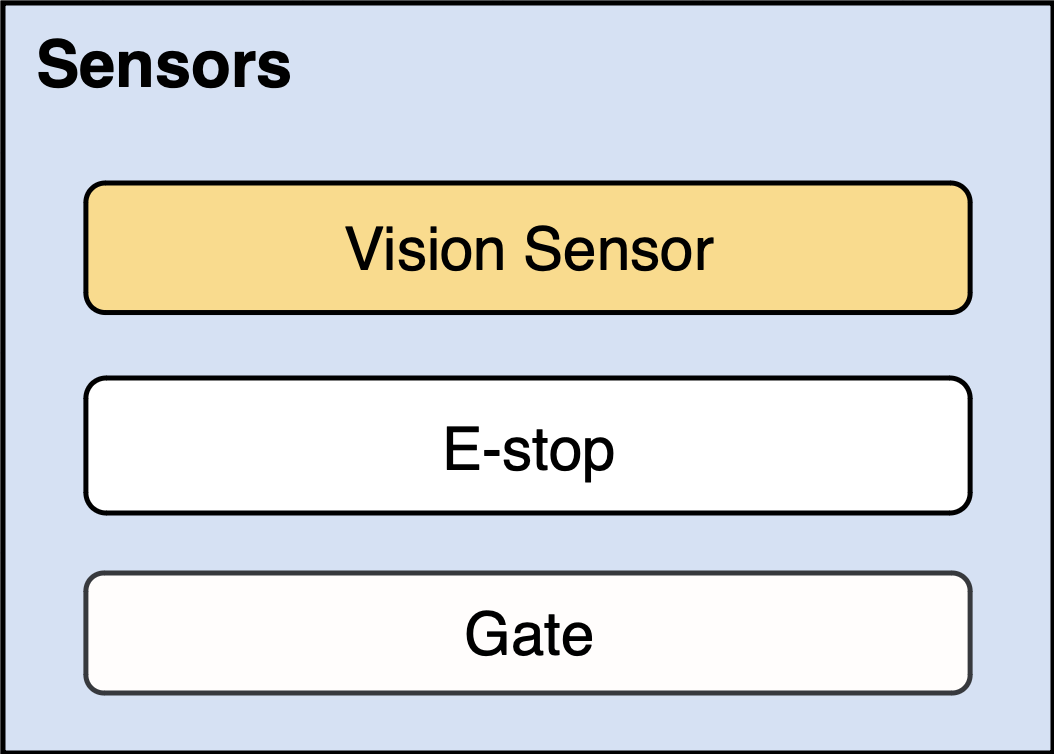
\includegraphics[width=0.60\textwidth]{images/vision}
 \caption{Vision subsystem diagram}
\end{figure}

\subsubsection{Subsystem Hardware}
A vision sensor will be mounted on the RV8 robot arm with a paintball gun.

\subsubsection{Subsystem Operating System}
Window 10 or 11

\subsubsection{Subsystem Software Dependencies}
Vision sensors will require software for configuration, calibration, data visualization, or integration with the robot control system, RT ToolBox 3 is a suitable option.

\subsubsection{Subsystem Programming Languages}
MELFA-BASIC IV programming language that is used by the Mitsubishi robots in the RT Toolbox 3 software.

\subsubsection{Subsystem Data Structures}
The information obtained from the vision sensor will be transmitted through the sensor to the PLC and to the connected computer.

\subsubsection{Subsystem Data Processing}
Extracts information from images or video streams captured by vision sensors.

\subsection{E-stop}
There will be multiple emergency stop (E-stop) buttons strategically placed throughout the system. These buttons will be located next to the case gate, on the controller, within an application (such as RT Toolbox) inside the cage, and alongside the linear rail. When any of these E-stop buttons are pressed, the entire system will immediately halt, ensuring rapid response to any safety concerns or emergencies.

\begin{figure}[h!]
	\centering
 	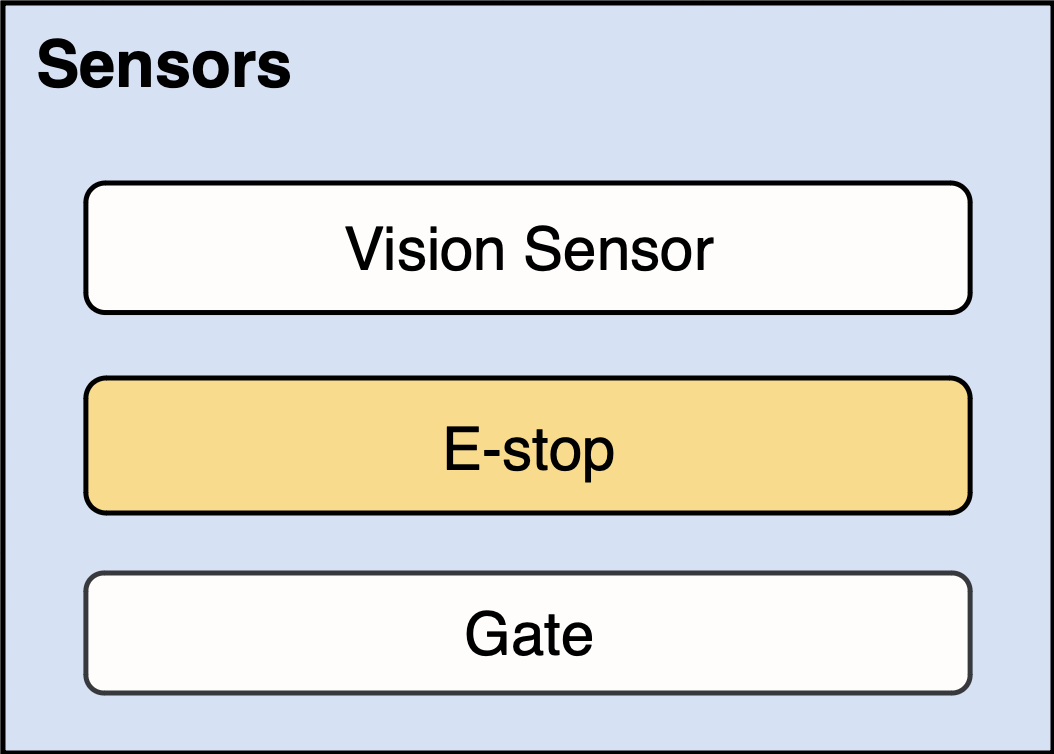
\includegraphics[width=0.60\textwidth]{images/E-stop}
 \caption{E-stop subsystem diagram}
\end{figure}

\subsubsection{Subsystem Hardware}
Inductive Proximity Sensors are used to limit the range of movement of the robot arm along the X-axis, E-stop sensors are utilized for emergency situations (True/False), and wires are employed to connect them to the PLC.

\subsubsection{Subsystem Operating System}
Window 10 or 11

\subsubsection{Subsystem Software Dependencies}
RT Toolbox 3 will be necessary to register the stop sensors.

\subsubsection{Subsystem Programming Languages}
MELFA-BASIC IV programming language

\subsubsection{Subsystem Data Structures}
True or False values from the physical stop sensor are sent to the PLC.

\subsubsection{Subsystem Data Processing}
capturing and analyzing signals generated when the emergency stop button or switch is pressed.

\subsection{Gate}
A contact sensor will be necessary to detect whether the gate is in closed or open position by physically making contact with the gate or its components. This is essential for safety measures to prevent the robot from damaging properties outside of the case.

\begin{figure}[h!]
	\centering
 	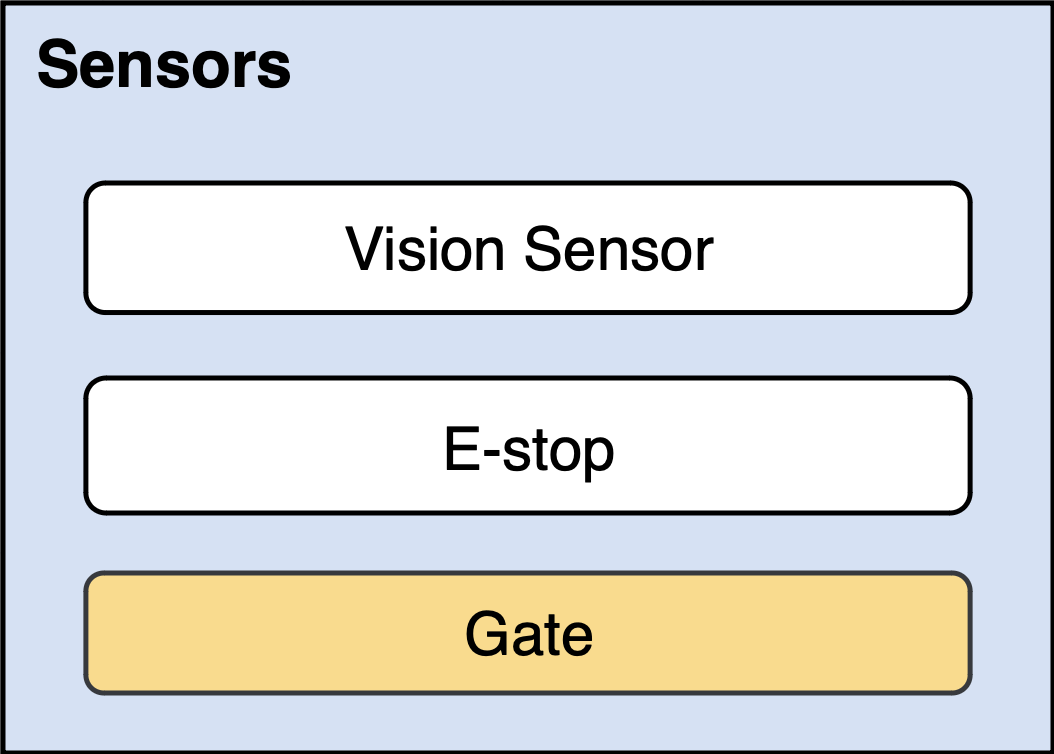
\includegraphics[width=0.60\textwidth]{images/Gate}
 \caption{Gate subsystem diagram}
\end{figure}

\subsubsection{Subsystem Hardware}
Contact sensors and PLCs need to be connected via wires to receive the signal.

\subsubsection{Subsystem Operating System}
Window 10 or 11

\subsubsection{Subsystem Software Dependencies}
RT Toolbox 3 will be necessary to register the contact sensors.

\subsubsection{Subsystem Programming Languages}
MELFA-BASIC IV programming language

\subsubsection{Subsystem Data Structures}
True or false values will be measured through the sensor, and this value will be transmitted to the PLC via wires.

\subsubsection{Subsystem Data Processing}
detects the physical contact or proximity of an object to a specific area, typically through the closure or opening of an electrical circuit.